\chapter{Bias-variance and ensembles}\label{ch-15}

SLT explained underfitting and overfitting through model complexity and
the number of data. The \textbf{bias-variance decomposition} offers
another, complementary point of view: it considers the fact that the
training set is \textbf{only one} of the possible realisations of the
data, and decomposes the expected error into three components ---
\textbf{bias}, \textbf{variance} and \textbf{noise}. From here we
naturally arrive at \textbf{ensembles} (bagging, boosting), which
exploit precisely the reduction of variance.

\section{The idea}\label{lidea}

A training set is only one possible realisation from the universe of
data: \textbf{different training sets produce different estimates}. The
expected error (over the various training sets) at a point
\(\mathbf{x}\) decomposes into:

\begin{itemize}
\tightlist
\item
  \textbf{Bias}: quantifies the discrepancy between the true function
  and \(h(\mathbf{x})\) (averaged over the data). It is high if \(H\) is
  too small (model too rigid).
\item
  \textbf{Variance}: quantifies the variability of the response of the
  model \(h\) for different realisations of the training data. It is
  due to excessive flexibility.
\item
  \textbf{Noise}: the labels contain a random error (for example, for a
  given \(\mathbf{x}\) there can be several possible values of \(d\)).
\end{itemize}

We assume the \textbf{regression} scenario with target \(y\) and
squared loss.

\section{Analysis in regression}\label{analisi-nella-regressione}

Suppose examples \(\langle \mathbf{x}, y\rangle\) with true function
\(y = f(\mathbf{x}) + \varepsilon\), where \(\varepsilon\) is Gaussian
noise with zero mean and standard deviation \(\sigma\). With linear
regression, given a set of examples \(\langle\mathbf{x}_i, y_i\rangle\),
\(i = 1..l\), a linear hypothesis \(h(\mathbf{x}) = \mathbf{w}\mathbf{x} + w_0\)
is fitted by minimising \(\sum_{i=1}^l (y_i - h(\mathbf{x}_i))^2\). Two
facts:

\begin{enumerate}
\def\labelenumi{\arabic{enumi}.}
\tightlist
\item
  for the chosen hypothesis class (linear), for some \(f\) there will
  be a \textbf{systematic prediction error};
\item
  depending on the dataset, the parameters \(\mathbf{w}\) found
  \textbf{will be different}.
\end{enumerate}

\begin{boxexample}{20 points and 50 fits}

True function \(y = x + 2\sin(1.5x) + \mathcal{N}(0; 0.2)\). With 20
points a line is fitted. Repeating with 50 different datasets (each of
20 points), 50 different lines are obtained.

\end{boxexample}

\begin{figure}[htbp]
\centering
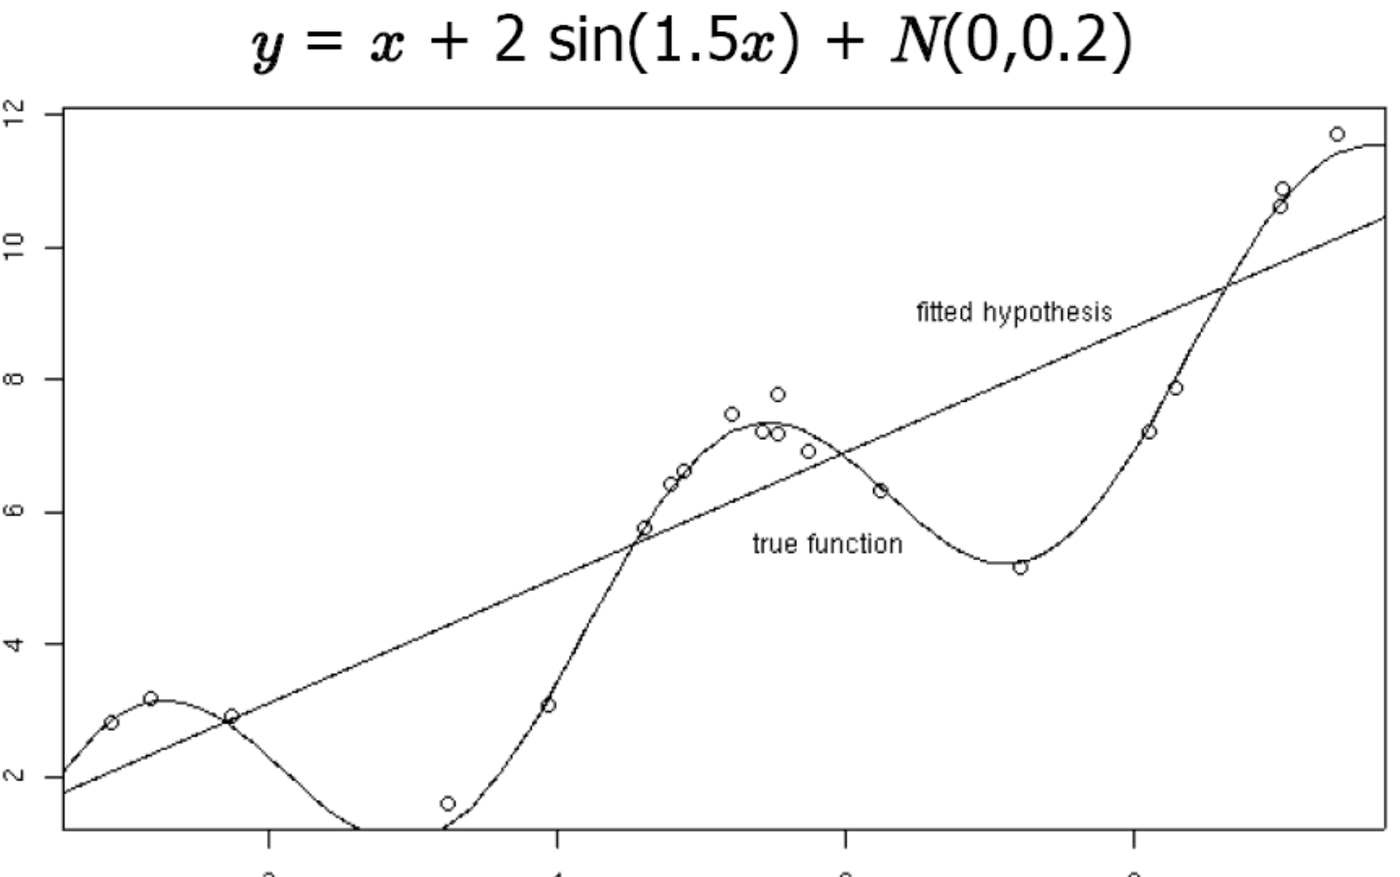
\includegraphics[width=0.63\linewidth,height=0.42\textheight,keepaspectratio]{images/15-bv_20punti.png}
\caption{A dataset of 20 points, the true function and the fitted linear
hypothesis.}
\end{figure}

\begin{figure}[htbp]
\centering
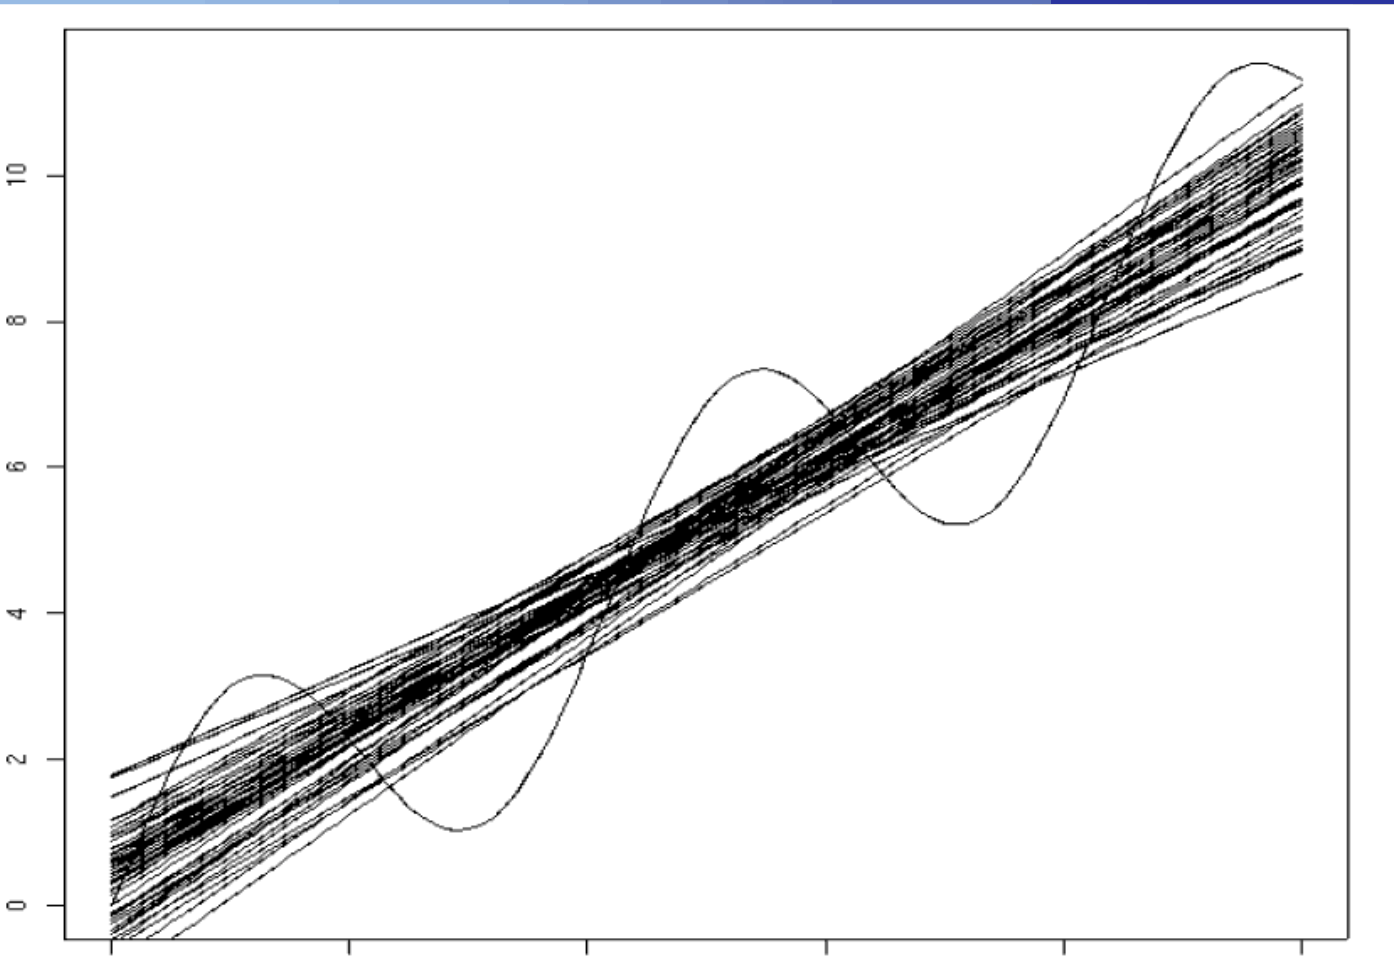
\includegraphics[width=0.63\linewidth,height=0.42\textheight,keepaspectratio]{images/15-bv_50fit.png}
\caption{50 fits, each on 20 points: the lines vary from one dataset to
another.}
\end{figure}

\subsection{The expected prediction
error}\label{lerrore-di-predizione-atteso}

Given a new point \(\mathbf{x}\), what is the \textbf{expected
prediction error}? The data are assumed to be drawn \textbf{i.i.d.}
(independent and identically distributed) from a single distribution
\(P\). The goal is to compute, for an arbitrary \(\mathbf{x}\), \[
E_P\big[(y - h(\mathbf{x}))^2\big],
\] where \(y\) is the value of \(\mathbf{x}\) that could appear in a
dataset, and the expectation is \textbf{over all training sets} drawn
according to \(P\). Beware: for each ``drawn'' training set there is a
different \(h\) (and a different \(y\)).

\subsection{Statistics recap}\label{richiamo-di-statistica}

For a discrete random variable \(Z\):
\(\bar Z = E_P[Z] = \sum_i z_i P(z_i)\) and
\(\operatorname{Var}[Z] = E[(Z - \bar Z)^2]\).

\begin{boxtheorem}{Variance lemma}

\[
\operatorname{Var}[Z] = E[Z^2] - \bar Z^2 \qquad\Longleftrightarrow\qquad E[Z^2] = \bar Z^2 + \operatorname{Var}[Z].
\] \textbf{Proof.}
\(\operatorname{Var}[Z] = \sum_i (z_i - \bar Z)^2 P(z_i) = \sum_i z_i^2P(z_i) - 2\bar Z\sum_i z_iP(z_i) + \bar Z^2\sum_i P(z_i) = E[Z^2] - 2\bar Z^2 + \bar Z^2 = E[Z^2] - \bar Z^2\).

\end{boxtheorem}

\subsection{The decomposition}\label{la-decomposizione}

Expanding the square and using the linearity of expectation (and the
fact that \(y\) and \(h(\mathbf{x})\) are independent, because \(y\) is
a new data point and \(h\) depends on the training set): \[
E_P\big[(y - h(\mathbf{x}))^2\big] = E_P\big[h(\mathbf{x})^2 - 2yh(\mathbf{x}) + y^2\big] = E_P\big[h(\mathbf{x})^2\big] + E_P\big[y^2\big] - 2E_P[y]\,E_P[h(\mathbf{x})].
\]

Let \(\bar h(\mathbf{x}) = E_P[h(\mathbf{x})]\) be the \textbf{mean
prediction} of the hypothesis at \(\mathbf{x}\), when \(h\) is trained
on data drawn from \(P\).

\begin{itemize}
\tightlist
\item
  \textbf{First term}, with the lemma:
  \(E_P[h(\mathbf{x})^2] = E_P\big[(h(\mathbf{x}) - \bar h(\mathbf{x}))^2\big] + \bar h(\mathbf{x})^2\).
\item
  Note that
  \(E_P[y] = E_P[f(\mathbf{x}) + \varepsilon] = f(\mathbf{x})\) (the
  noise has zero mean).
\item
  \textbf{Second term}, with the lemma:
  \(E_P[y^2] = E_P\big[(y - f(\mathbf{x}))^2\big] + f(\mathbf{x})^2\).
\end{itemize}

Putting everything together: \[
\begin{aligned}
E_P\big[(y - h(\mathbf{x}))^2\big] &= E_P\big[(h(\mathbf{x}) - \bar h(\mathbf{x}))^2\big] + \underbrace{\bar h(\mathbf{x})^2 - 2f(\mathbf{x})\bar h(\mathbf{x}) + f(\mathbf{x})^2}_{(\bar h(\mathbf{x}) - f(\mathbf{x}))^2} + E_P\big[(y - f(\mathbf{x}))^2\big] \\
&= \underbrace{E_P\big[(h(\mathbf{x}) - \bar h(\mathbf{x}))^2\big]}_{\text{variance}} + \underbrace{\big(\bar h(\mathbf{x}) - f(\mathbf{x})\big)^2}_{\text{bias}^2} + \underbrace{E_P\big[(y - f(\mathbf{x}))^2\big]}_{\text{noise}^2} \\
&= \operatorname{Var}[h(\mathbf{x})] + \operatorname{Bias}[h(\mathbf{x})]^2 + E_P[\varepsilon^2] = \operatorname{Var}[h(\mathbf{x})] + \operatorname{Bias}[h(\mathbf{x})]^2 + \sigma^2.
\end{aligned}
\]

\begin{boxtheorem}{Bias-variance decomposition}

\[
\text{Expected prediction error} = \text{Variance} + \text{Bias}^2 + \text{Noise}^2.
\]

\end{boxtheorem}

\subsection{Interpretation of the three
components}\label{interpretazione-delle-tre-componenti}

\begin{itemize}
\tightlist
\item
  \textbf{Bias} \(\big(\bar h(\mathbf{x}) - f(\mathbf{x})\big)^2\): the
  discrepancy between the true function and the \textbf{mean}
  prediction over the different training sets. It is a
  \textbf{systematic error}, due for example to a space \(H\) that is
  too small or a model that is too rigid.
\item
  \textbf{Variance}: the variability of the response of the model for
  different realisations of the training set. It is due to
  \textbf{excessive flexibility}.
\item
  \textbf{Noise}: even the optimal solution can be wrong (for example
  if for a given \(\mathbf{x}\) several values of \(d\) are possible).
  It is \textbf{irreducible}: it does not depend on the model and
  represents a tolerance on the response (\(\sigma\)).
\end{itemize}

\begin{figure}[htbp]
\centering
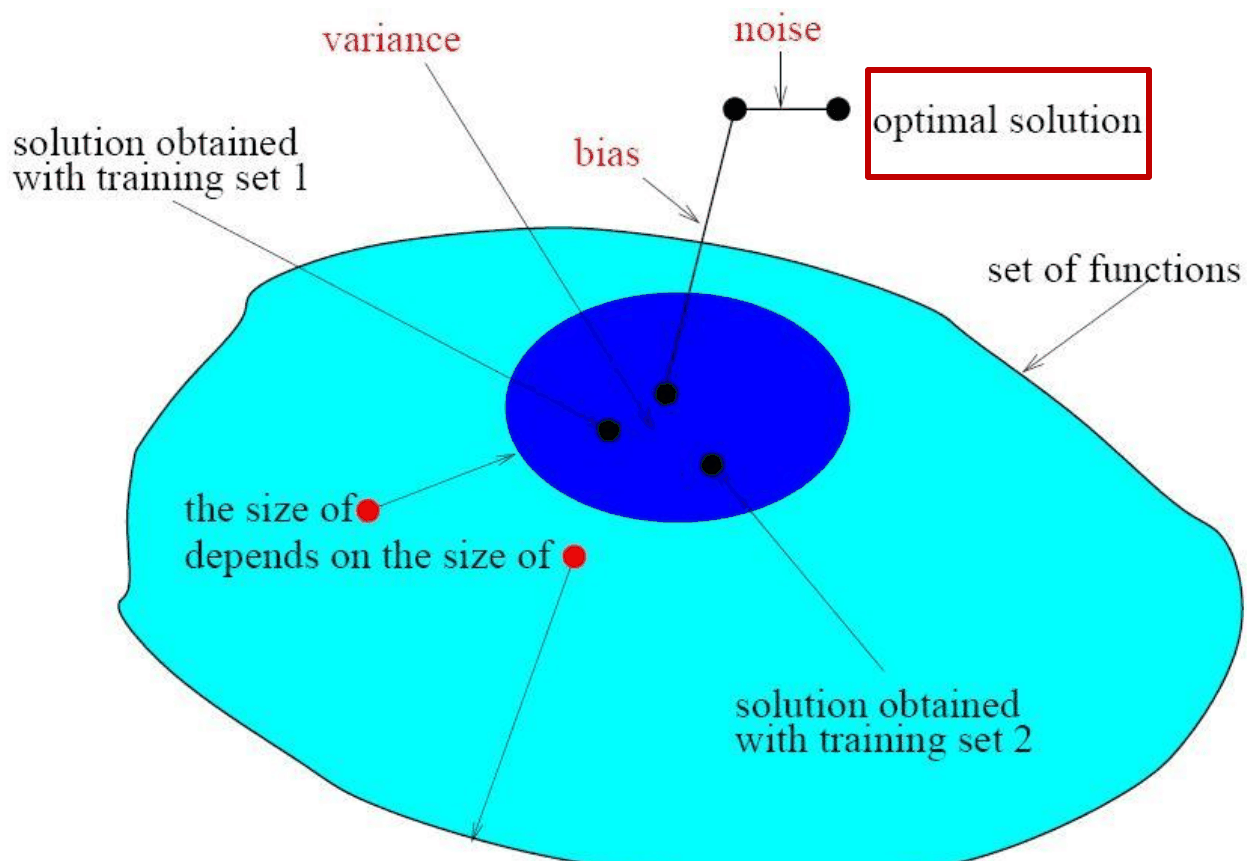
\includegraphics[width=0.66\linewidth,height=0.42\textheight,keepaspectratio]{images/15-bv_vista-grafica.png}
\caption{Graphical view: different training sets produce different
solutions (variance); their mean is far from the optimum (bias); the
optimum itself is far from the data because of noise.}
\end{figure}

Going back to the example: the \textbf{bias} is evident in the mean
\(\bar h\) of the 50 lines, which remains far from the wavy true
function (the linear model is too rigid); the \textbf{variance} is the
spread of the 50 lines around \(\bar h\); the \textbf{noise} is the
spread of the data around the true function.

\begin{figure}[htbp]
\centering
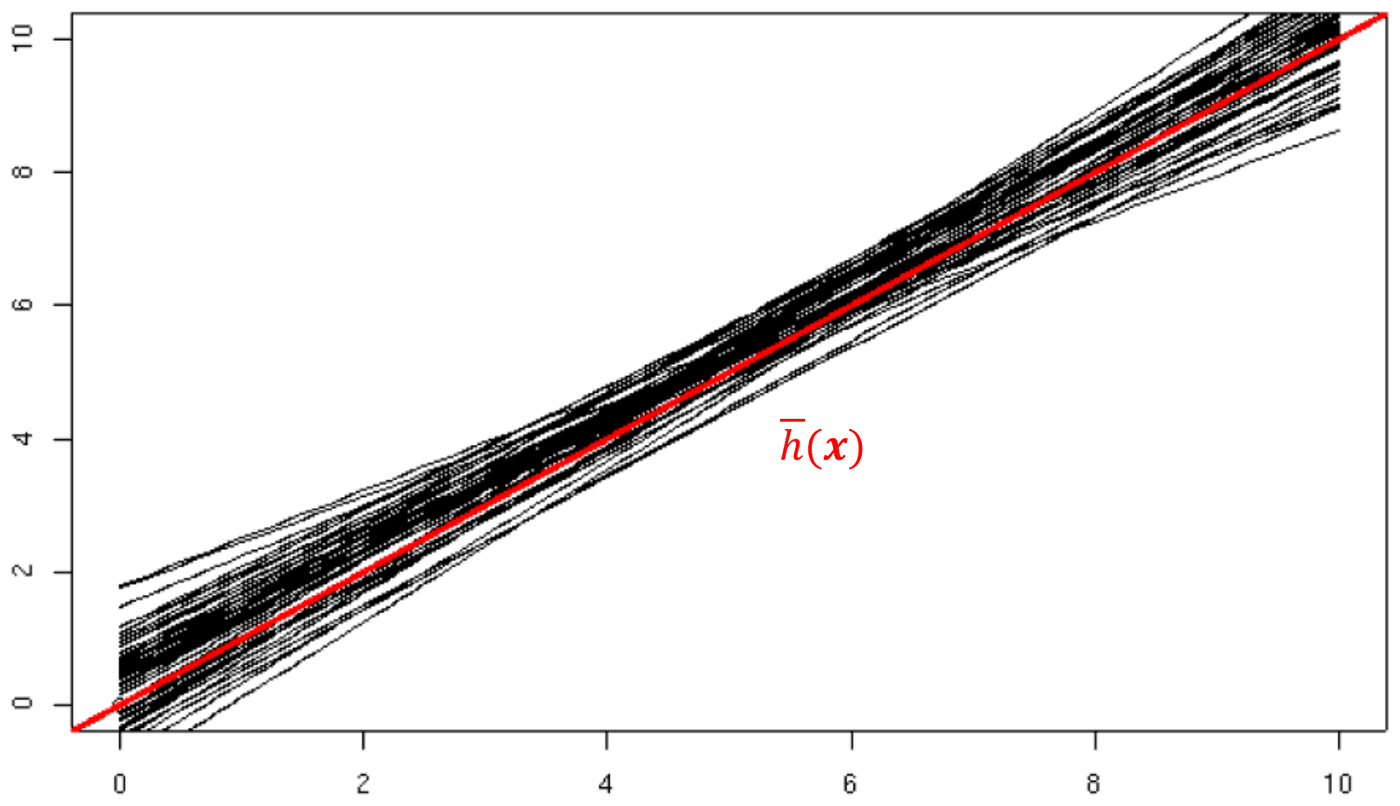
\includegraphics[width=0.63\linewidth,height=0.42\textheight,keepaspectratio]{images/15-bv_varianza.png}
\caption{The variance: the spread of the hypotheses around the mean
prediction \(\bar h(\mathbf{x})\) (in red).}
\end{figure}

\begin{boxexample}{The darts analogy}

\begin{center}
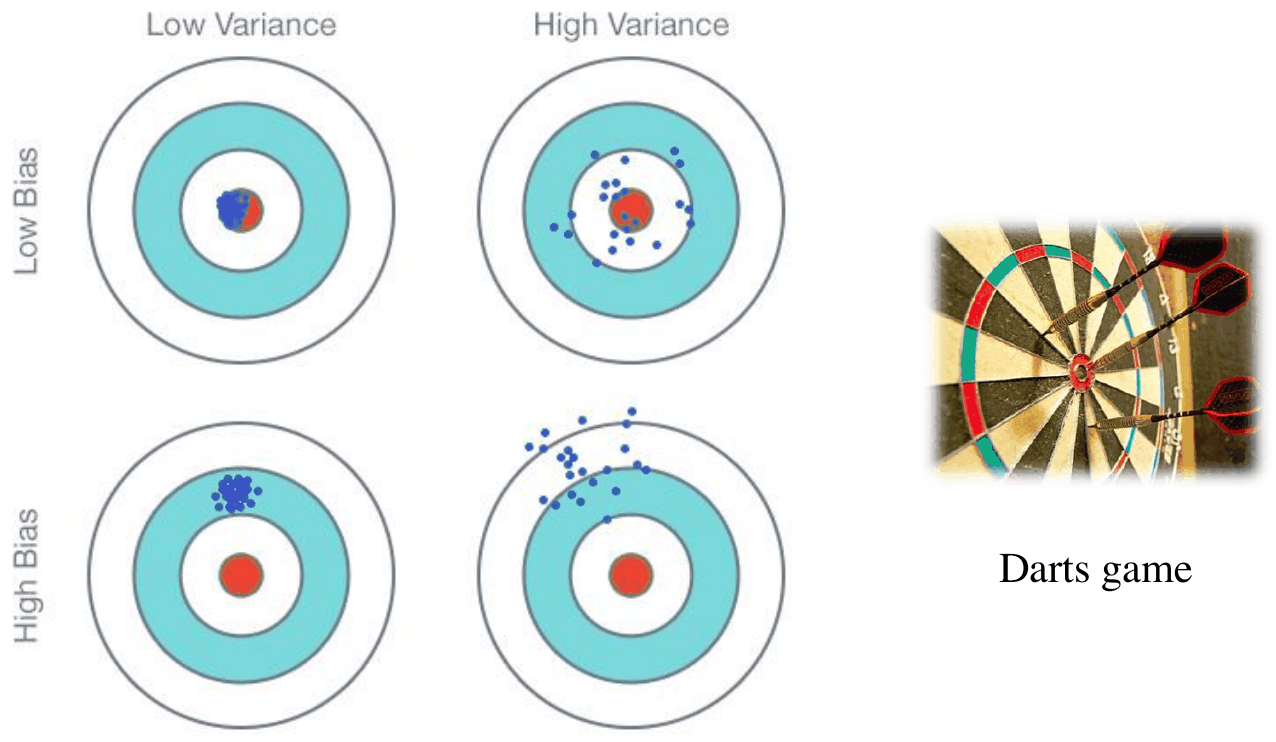
\includegraphics[width=0.63\linewidth,height=0.42\textheight,keepaspectratio]{images/15-bv_freccette.png}
\end{center}

The centre is the true function, each dart is a model trained on a
different training set. \textbf{High bias and low variance} (bottom
left) corresponds to \textbf{underfitting}; \textbf{low bias and high
variance} (top right) to \textbf{overfitting}. The analogy is not
perfect for ML, but it helps.

\end{boxexample}

\section{Bias, variance and
regularisation}\label{bias-varianza-e-regolarizzazione}

Recall the regularised loss: \[
\text{Loss}(\mathbf{w}) = \underbrace{\sum_p\big(d_p - o(\mathbf{x}_p)\big)^2}_{\text{data term}} + \underbrace{\lambda\|\mathbf{w}\|^2}_{\text{penalty}}.
\] Varying \(\lambda\) we obtain less regularised solutions (complex,
low \(\lambda\)) or more regularised ones (less complex, high
\(\lambda\)). (The intercept is typically excluded from the penalty.)

Bishop's example: 25 datasets drawn from the sinusoid, a model (an RBF
network) trained on each with different values of \(\lambda\).

\begin{figure}[htbp]
\centering
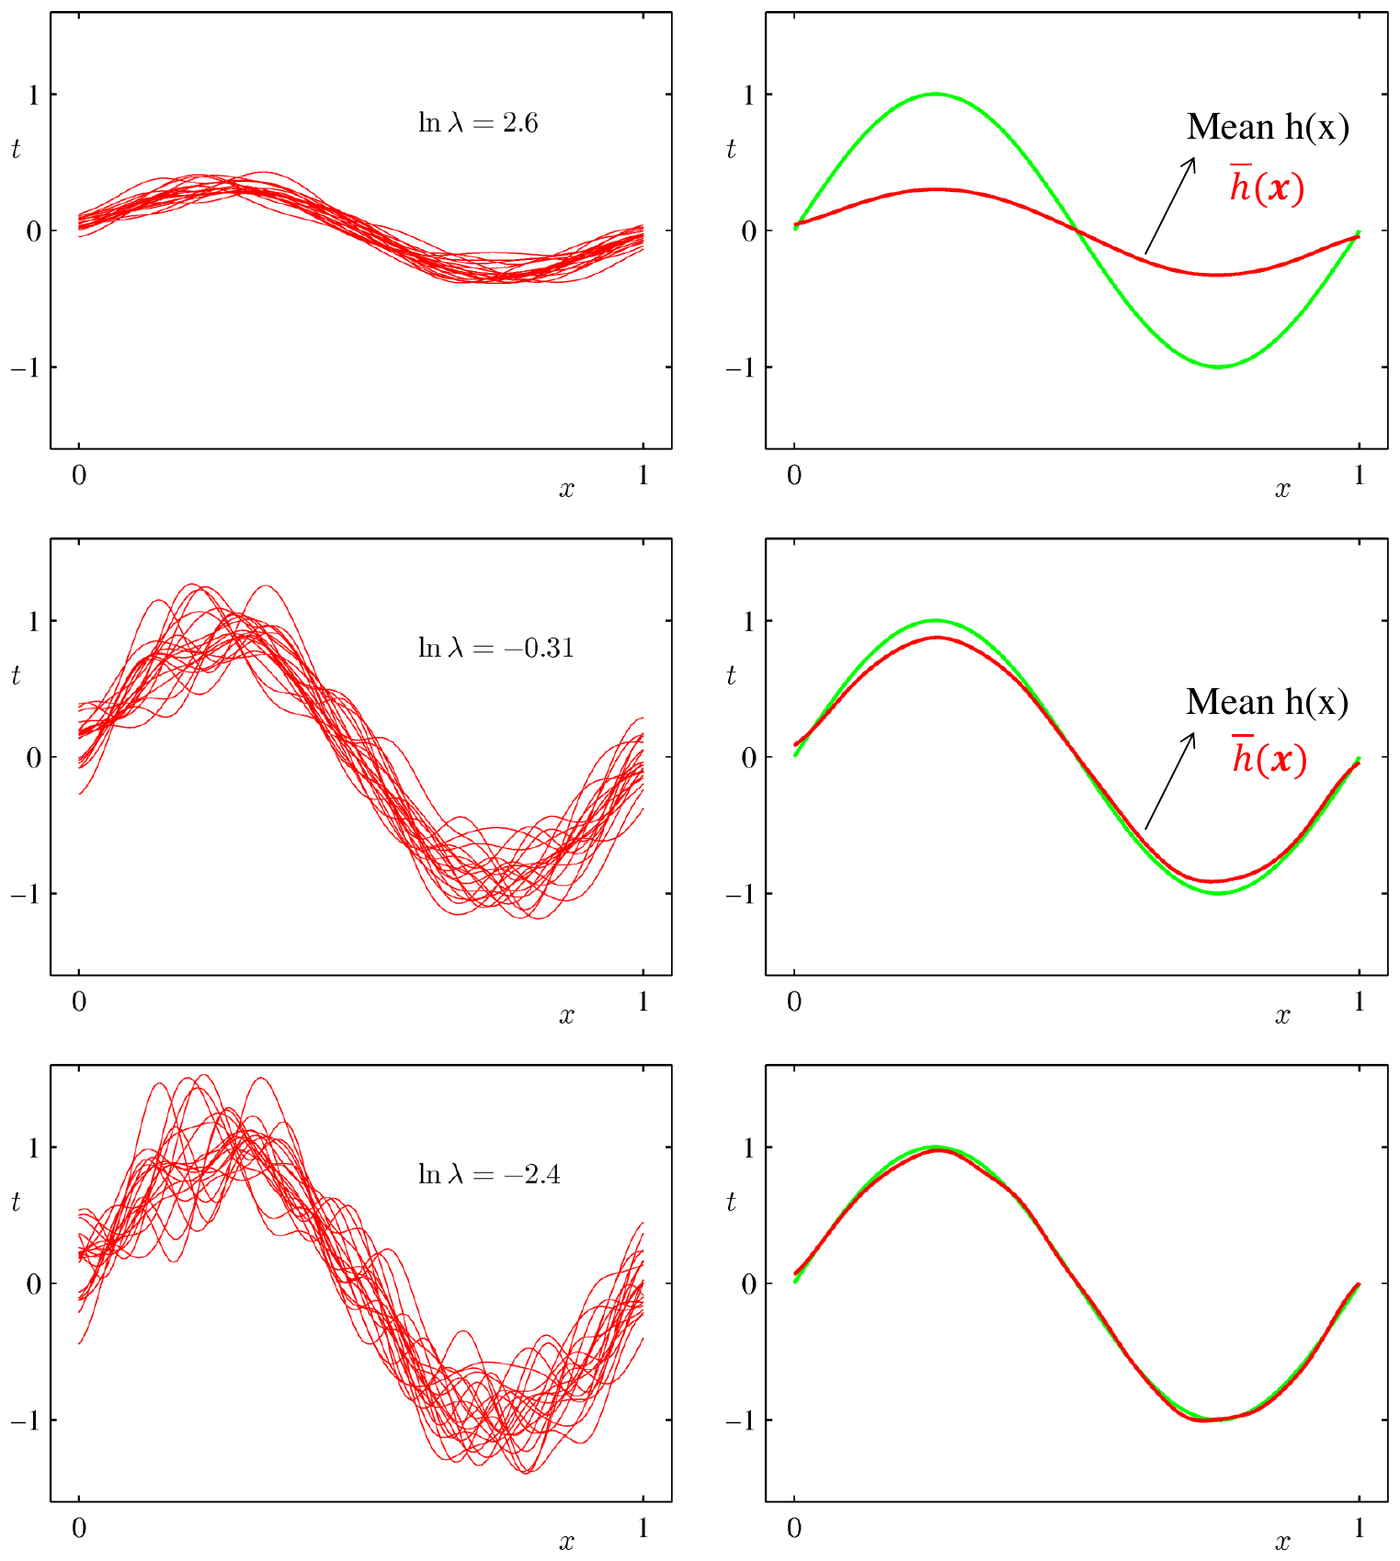
\includegraphics[width=0.80\linewidth,height=0.42\textheight,keepaspectratio]{images/15-bv_lambda.png}
\caption{Effect of \(\lambda\) on bias and variance: \(\ln\lambda = 2.6\)
(top), \(-0.31\) (middle), \(-2.4\) (bottom). On the left the 25
hypotheses, on the right their mean \(\bar h(x)\) (red) and the true
function (green).}
\end{figure}

\begin{itemize}
\tightlist
\item
  \textbf{High \(\lambda\)}: \textbf{high bias, low variance}. The
  penalty dominates, the model depends little on the data and is ``too
  rigid'': the curves are similar but their mean is far from the
  sinusoid.
\item
  \textbf{Medium \(\lambda\)}: lower bias, higher variance. Decreasing
  \(\lambda\) one depends more on the particular training set.
\item
  \textbf{Very low \(\lambda\)}: \textbf{low bias, high variance}. The
  test error for a single training set can be high (because of the
  variance component), but even though the curves are very different
  from each other, \textbf{on average} they are correct (plot on the
  right).
\end{itemize}

\begin{figure}[htbp]
\centering
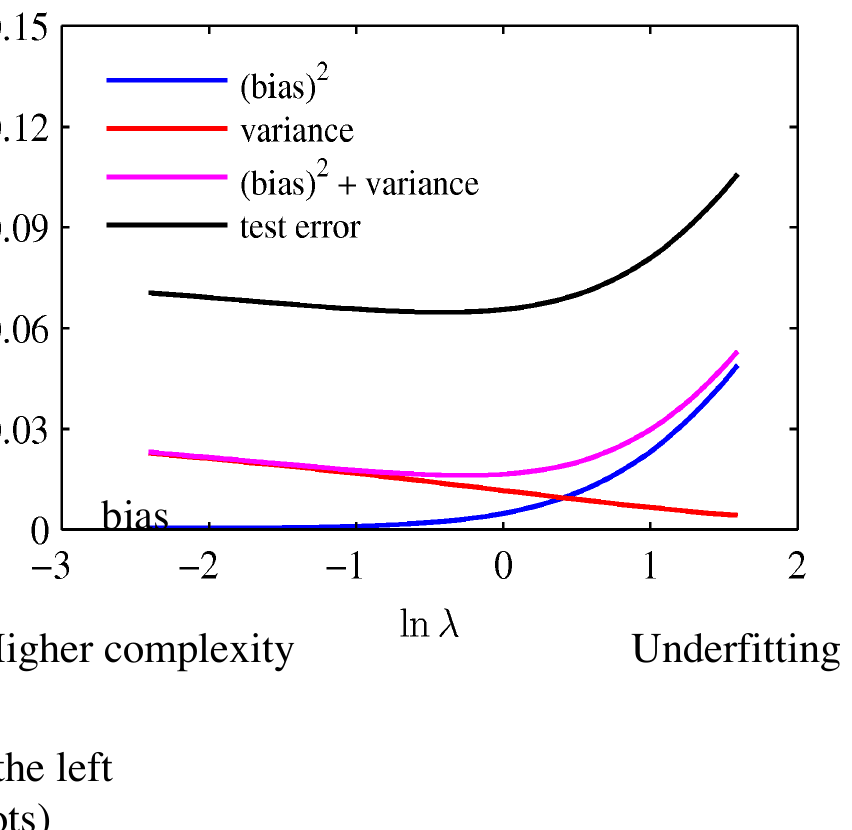
\includegraphics[width=0.51\linewidth,height=0.42\textheight,keepaspectratio]{images/15-bv_tradeoff.png}
\caption{The bias-variance trade-off as \(\ln\lambda\) varies. Beware:
here complexity is higher on the \textbf{left} (the opposite of the
usual plots).}
\end{figure}

An \textbf{over-regularised} model (large \(\lambda\)) has high bias;
an \textbf{under-regularised} one (small \(\lambda\)) has high
variance. Again, \textbf{the trade-off}: the minimum of bias² +
variance roughly coincides with the minimum of the test error.

The same figure seen in validation
(\href{09\%20-\%20Validazione\%20(parte\%201)\%20-\%20model\%20selection\%20e\%20assessment}{09
- Validation (part 1) - model selection and assessment}) shows, as
complexity grows, training and test errors on 100 training sets: a
complex model has \textbf{low bias and high variance}, hence a risk of
overfitting, and depending on the training set one can be lucky or
unlucky.

\begin{boxtip}{The link with SLT}

Bias and variance are another face of the trade-off between fitting
the data and complexity: bias corresponds to the inability of the model
to represent the function (high \(R_{emp}\), underfitting), variance to
the sensitivity to the specific data (high VC-confidence,
overfitting).

\end{boxtip}

\section{Ensemble learning}\label{ensemble-learning}

The idea of \textbf{ensembles} is to exploit \textbf{several models} by
combining their responses.

In the simplest case (\textbf{voting scheme}):

\begin{itemize}
\tightlist
\item
  \textbf{Regression}: simple averaging committee,
  \(o(\mathbf{x}) = \frac{1}{K}\sum_{i=1}^K h_i(\mathbf{x})\).
\item
  \textbf{Classification}: vote over many classifiers (as long as they
  give \textbf{diversified} answers), or classify after averaging the
  continuous outputs.
\end{itemize}

Alternatively (\textbf{stacking}) the combiner is itself an ML model.

\begin{boxtheorem}{The committee is not worse than the average of its members}

For a convex loss such as the squared error, the error of the committee
is less than or equal to the average of the errors of the individual
models: \[
\text{loss}\big(E_i[h_i]\big) \le E_i\big[\text{loss}(h_i)\big].
\] (It is Jensen's inequality.) Example with target \(t = 5\) and two
models predicting 2 and 4: the average of the errors is
\(\frac{(5-2)^2 + (5-4)^2}{2} = 5\), while the error of the committee
(\(o = 3\)) is \((5-3)^2 = 4\). With predictions 6 and 4: average of
the errors \(\frac{1 + 1}{2} = 1\), committee error \((5-5)^2 = 0\).

\end{boxtheorem}

\subsection{Bagging (bootstrap
aggregating)}\label{bagging-bootstrap-aggregating}

\begin{itemize}
\tightlist
\item
  \(K\) classifiers are trained on \textbf{different subsets} of the
  training set, differentiated with the \textbf{bootstrap} (resampling
  with replacement).
\item
  Regression: the average is used; classification: vote of the \(K\)
  classifiers.
\end{itemize}

The link with bias-variance is direct (recall the ``low \(\lambda\)''
case): \textbf{high-variance} and \textbf{low-bias} models can work
well \textbf{on average}. In other words, \textbf{averaging the \(h\)
reduces variance} without increasing bias. Moreover bagging tends to
increase the \textbf{margin} of a classifier: the average of \(K\)
separation curves tends to lie ``in the middle'' (\emph{in medio stat
virtus}).

\subsection{Boosting (e.g.\ AdaBoost)}\label{boosting-es.-adaboost}

If the models make the \textbf{same errors}, combining them is useless.
Boosting differentiates them on purpose:

\begin{enumerate}
\def\labelenumi{\arabic{enumi}.}
\tightlist
\item
  it trains the classifiers in sequence focusing on the
  \textbf{errors}: the second gives more weight to the instances
  misclassified by the first (for example they are more likely in its
  training set), and so on;
\item
  it combines the results with a \textbf{weighted vote}, giving more
  weight to the classifiers with lower error.
\end{enumerate}

If not stopped, boosting learns to correctly classify \textbf{all} the
training instances using \textbf{weak learners} (classifiers just
better than chance, with error \(< 1/2\) in the binary case),
incrementally building complex models. It can greatly improve the
performance of weak learners; it reduces bias without increasing
variance (it resists overfitting) and, like bagging, it tends to
produce separation curves ``in the middle'' (maximum margin). However,
it \textbf{suffers with noisy data} (which are weighted more and more),
and it does not by itself solve the underfitting/overfitting problem.

\section{Feature selection (outline)}\label{feature-selection-cenni}

Finding the subset of the most informative features for the problem
brings great benefits: \textbf{dimensionality reduction} (effects on
the VC-dim of networks, on the curse of dimensionality\ldots),
filtering of irrelevant information and noise (with possibly strong
performance improvements), \textbf{interpretability} (finding useful
descriptors). But:

\begin{itemize}
\tightlist
\item
  it is \textbf{computationally hard} (huge number of possible subsets,
  and each evaluation requires retraining);
\item
  a \textbf{heuristic search} is typically used (greedy, genetic
  algorithms or other optimisation techniques), including the learner
  or not;
\item
  the results are particularly sensitive to the validation method:
  beware of the \textbf{feature subset selection bias}, i.e.\ the error
  of making the selection on the whole dataset (see the slides on
  cross-validation).
\end{itemize}

Other related topics: PAC learning; comparison between inductive
principles (SRM, MDL, Bayesian inference, regularisation) with respect
to complexity control.

\begin{boxabstract}{Summary}

The expected error (over training sets) decomposes into
\textbf{variance + bias² + noise}. Rigid (or heavily regularised)
models have high bias and low variance (underfitting); flexible
(lightly regularised) models have low bias and high variance
(overfitting); noise is irreducible. \textbf{Ensembles} exploit the
decomposition: \textbf{bagging} averages high-variance models, reducing
it; \textbf{boosting} combines weak learners by focusing on errors.

\end{boxabstract}

\begin{boxquestion}{Possible exam questions}

\begin{itemize}
\tightlist
\item
  Derive the bias-variance decomposition for the squared loss.
\item
  What do bias, variance and noise represent? Which component is
  irreducible?
\item
  How do bias and variance vary with the regularisation parameter
  \(\lambda\)?
\item
  Why is a committee not worse than the average of its members?
\item
  Difference between bagging and boosting; why does bagging reduce
  variance?
\end{itemize}

\end{boxquestion}
